\documentclass[10pt,twocolumn]{article}

\usepackage[margin=0.75in]{geometry}
\usepackage[T1]{fontenc}
\usepackage[utf8]{inputenc}
\usepackage{lmodern}
\usepackage{microtype}
\usepackage{graphicx}
\usepackage{booktabs}
\usepackage{array}
\usepackage{url}
\usepackage[hidelinks]{hyperref}
\usepackage[numbers]{natbib}
\setlength{\columnsep}{0.24in}

\title{Detecting Political Bias in News Articles Using Deep Learning:\\
From BiLSTM to Ordinal DistilRoBERTa}

\author{
Kellin Harris \and
Lasya Suravajhela \and
Michael Long \and
Prashant Joshi \and
Tracey Peyton\\
University of Washington
}

\date{Spring 2026}

\begin{document}
\maketitle

\begin{abstract}
We study whether the political leaning of a news article can be predicted from
article text alone, without relying on source identity. Using the
Article-Bias-Prediction dataset, which contains labeled left, center, and right
news articles, we compare two supervised classifiers: a bidirectional LSTM with
a learned embedding layer and an ordinal DistilRoBERTa classifier with
cumulative ordinal targets. The BiLSTM baseline reaches 61.4\% test accuracy,
above the random baseline of 33.3\%. The ordinal DistilRoBERTa model improves
test accuracy to 71.9\% and obtains balanced F1 scores of 0.71, 0.72, and 0.72
for left, center, and right articles, respectively. We also evaluate
generalization qualitatively on a newly collected set of articles from BBC,
ABC, CBC, FOX, Al Jazeera, and NPR. The BiLSTM model exhibits a notable
failure mode on FOX articles, often labeling them as left-leaning, whereas the
ordinal DistilRoBERTa model shifts FOX predictions toward the expected
right-leaning category. These results suggest that article-level political
leaning can be learned from text, but robust generalization depends on both
training-source diversity and representation quality.
\end{abstract}

\section{Introduction}

Political bias in news is widely perceived by readers and has consequences for
both public interpretation and downstream machine-learning systems trained on
news corpora. Many existing bias resources, such as outlet-level media-bias
charts, classify sources as a whole. However, outlet-level labels can be too
coarse for article-level analysis: a right-leaning outlet may publish neutral
reporting, and a centrist outlet may publish opinion-heavy pieces.

This project asks whether political leaning can be inferred from article text
alone. Motivated by the distributional hypothesis, we assume that word choice,
framing, and local context can reveal ideological slant even when source
metadata is withheld. We compare a sequence model trained from scratch against
a transformer model with pretrained contextual representations, and we evaluate
whether ordinal encoding better reflects the left--center--right spectrum.

\section{Related Work}

Source-level political leaning and factuality prediction have been studied by
\citet{baly2018predicting}, who combined textual and source metadata signals.
The Article-Bias-Prediction dataset introduced by \citet{baly2020detect} is the
primary labeled article-level resource used in this project. Transformer-based
political-bias detection has also been explored in later work, including
ChunkyBERT \citep{loiya2026chunkybert}, while word-embedding approaches have
been used to analyze ideological placement in political text
\citep{rheault2019word}. Hybrid transformer-recurrent architectures have shown
promise in related sentiment tasks \citep{tan2022roberta}.

We also reference the Hugging Face model card
\texttt{matous-volf/political-leaning-politics}, which documents a
left/center/right political-leaning classifier based on the POLITICS model and
a combined training corpus that includes Article Bias Prediction
\citep{huggingfacepolitics}. That card is marked with the CC-BY-NC-4.0 license;
this manuscript cites it for provenance and related framing.

\section{Data}

\subsection{Training Dataset}

The Article-Bias-Prediction dataset contains news articles with article-level
political leaning labels. Each record includes fields such as title, source,
URL, publication date, article content, and bias label. The report describes
37,554 available articles; the train, validation, and test split files used in
the project account for the subset shown in Table~\ref{tab:splits}.

\begin{table}[h]
\centering
\caption{Article-Bias-Prediction split statistics used in the experiments.}
\label{tab:splits}
\begin{tabular}{lrrrr}
\toprule
Split & Left & Center & Right & Total \\
\midrule
Train & 9750 & 7988 & 10240 & 27978 \\
Validation & 2438 & 1998 & 2560 & 6996 \\
Test & 402 & 299 & 599 & 1300 \\
\midrule
Total & 12590 & 10285 & 13399 & 36274 \\
\bottomrule
\end{tabular}
\end{table}

The labels are reasonably balanced: right articles form the largest class,
followed by left and center. The average article length is approximately 1084
words, with broad variation across documents.

\subsection{Real-World Evaluation Corpus}

To qualitatively evaluate generalization, we collected a real-world article
corpus from six major news outlets: BBC, ABC, CBC, FOX, Al Jazeera, and NPR.
The written report describes a 1990-article evaluation corpus. The repository
also contains a later consolidated working folder with duplicate pulls and
list-style JSON payloads; the reproducibility notes in the repository README
document the distinction between raw files, unique URLs, and prediction rows.
Because the real-world corpus lacks ground-truth labels, these experiments are
interpreted as qualitative generalization checks rather than strict accuracy
tests.

\section{Methods}

\subsection{Experiment 1: Bidirectional LSTM Baseline}

The first model is a BiLSTM classifier implemented in TensorFlow/Keras. Article
text is lowercased, stripped of URLs, email addresses, special characters, and
digits, and normalized for whitespace. A Keras tokenizer is fit on the training
corpus with a vocabulary of 5000 tokens. Articles are padded or truncated to
500 tokens.

The model architecture consists of a learned embedding layer with 128
dimensions, dropout, two bidirectional LSTM layers with 64 units, two dense
layers with ReLU activations and dropout, and a final three-way softmax output.
Training uses Adam with learning rate 0.001, sparse categorical cross entropy,
and early stopping on validation loss.

\subsection{Experiment 2: Ordinal DistilRoBERTa}

The second model treats political leaning as an ordered spectrum rather than an
unordered set of classes. Labels are encoded as cumulative ordinal targets:
left as $(1,0,0)$, center as $(1,1,0)$, and right as $(1,1,1)$. During
inference, each logit is passed through a sigmoid; active bits above threshold
0.5 are counted to recover the predicted class.

The encoder is \texttt{distilroberta-base}. The final transformer-layer CLS
embedding is passed through dropout with rate 0.1 and a linear head producing
three ordinal logits. The model is trained with binary cross entropy over the
ordinal bits. In addition to accuracy and F1 score, we report ordinal mean
absolute error (MAE), ordinal mean squared error (MSE), and severe error rate,
where severe errors are opposite-pole mistakes.

\section{Results}

\subsection{BiLSTM Baseline}

The BiLSTM converged with early stopping and achieved 61.4\% test accuracy on
7511 held-out examples. Per-class metrics are shown in
Table~\ref{tab:lstm-results}. The center class was the hardest class, with an
F1 score of 0.58.

\begin{table}[h]
\centering
\caption{BiLSTM per-class performance.}
\label{tab:lstm-results}
\begin{tabular}{lrrrr}
\toprule
Class & Precision & Recall & F1 & Support \\
\midrule
Left & 0.62 & 0.61 & 0.61 & 2601 \\
Center & 0.65 & 0.52 & 0.58 & 2163 \\
Right & 0.59 & 0.70 & 0.64 & 2747 \\
\midrule
Macro avg. & 0.62 & 0.61 & 0.61 & 7511 \\
\bottomrule
\end{tabular}
\end{table}

\subsection{Ordinal DistilRoBERTa}

The ordinal DistilRoBERTa model reached 71.9\% accuracy on the 1300-example
test set. Per-class performance is shown in Table~\ref{tab:roberta-results}.
The model improved all three F1 scores relative to the BiLSTM baseline.

\begin{table}[h]
\centering
\caption{Ordinal DistilRoBERTa per-class performance.}
\label{tab:roberta-results}
\begin{tabular}{lrrrr}
\toprule
Class & Precision & Recall & F1 & Support \\
\midrule
Left & 0.76 & 0.67 & 0.71 & 402 \\
Center & 0.58 & 0.96 & 0.72 & 299 \\
Right & 0.85 & 0.63 & 0.72 & 599 \\
\midrule
Macro avg. & 0.73 & 0.76 & 0.72 & 1300 \\
\bottomrule
\end{tabular}
\end{table}

Distance-aware metrics further characterize the ordinal behavior: ordinal MAE
was 0.390 on a 0--2 scale, ordinal MSE was 0.608, and severe error rate was
10.9\%.

\begin{table}[h]
\centering
\small
\setlength{\tabcolsep}{3pt}
\caption{Summary comparison of the two final models.}
\label{tab:comparison}
\begin{tabular}{@{}lccccc@{}}
\toprule
Model & Acc. & L-F1 & C-F1 & R-F1 & Sev. \\
\midrule
BiLSTM & 0.614 & 0.61 & 0.58 & 0.64 & -- \\
Ord. RoBERTa & 0.719 & 0.71 & 0.72 & 0.72 & 0.109 \\
\bottomrule
\end{tabular}
\end{table}

\subsection{Real-World Generalization}

The real-world evaluation highlights an important failure mode of the BiLSTM.
On FOX articles, the BiLSTM classified 51.4\% as left and only 11.6\% as right.
The ordinal DistilRoBERTa model reversed this pattern, classifying 74.9\% of
FOX articles as right and 8.5\% as left. NPR predictions also shifted toward
center, from 31.3\% center under BiLSTM to 64.7\% center under RoBERTa.

\begin{table}[h]
\centering
\small
\setlength{\tabcolsep}{4pt}
\caption{Real-world source prediction comparison.}
\label{tab:realworld}
\begin{tabular}{@{}lcc@{}}
\toprule
Metric & BiLSTM & Ord. RoBERTa \\
\midrule
FOX right share & 11.6\% & 74.9\% \\
FOX left share & 51.4\% & 8.5\% \\
NPR center share & 31.3\% & 64.7\% \\
\bottomrule
\end{tabular}
\end{table}

\begin{figure}[h]
\centering
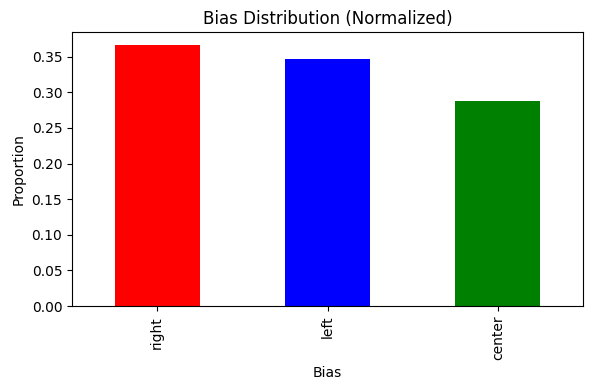
\includegraphics[width=0.72\linewidth]{figures/report_figure_1.png}
\caption{Normalized label distribution for the Article-Bias-Prediction training
data.}
\label{fig:label-distribution}
\end{figure}

\section{Discussion}

Both models perform substantially above chance, suggesting that political
leaning can be predicted from article text. The RoBERTa improvement indicates
that pretrained contextual representations are better suited to the task than
embeddings learned from scratch. The ordinal model also provides more
interpretable distance-aware metrics: most mistakes are adjacent-class errors
rather than opposite-pole errors.

The BiLSTM's FOX behavior illustrates a deployment risk. A model trained on a
narrow set of sources may learn superficial source- or topic-specific language
patterns instead of robust ideological cues. The ordinal DistilRoBERTa model
mitigates this particular failure, but the broader issue remains: source
coverage and label provenance strongly shape model behavior.

\section{Limitations and Ethics}

The label scheme is reductive. Political ideology is multidimensional, and
left, center, and right categories may not capture religious conservatism,
green politics, libertarianism, or international ideological structures.
Dataset labels are inherited from external media-bias assessments, so source
labeling uncertainty propagates into article-level labels.

The transformer model processes only 128 tokens per article, which means much
of each article is omitted. Future work should explore chunking, hierarchical
encoding, longer-context models, confidence calibration, and broader source
coverage. Any deployed classifier should present predictions probabilistically,
document training data limitations, and avoid definitive claims about an
article's ideology.

\section{Conclusion}

This work provides a reproducible baseline for article-level political-bias
classification and a documented upgrade path from a BiLSTM sequence model to an
ordinal transformer classifier. The BiLSTM achieved 61.4\% test accuracy, while
the ordinal DistilRoBERTa model achieved 71.9\% and improved F1 scores across
all classes. The real-world source evaluation underscores both the promise and
the risk of text-only political-bias classifiers: stronger representations help,
but robust generalization requires broader training data and careful
interpretation.

\bibliographystyle{plainnat}
\bibliography{references}

\end{document}
